%% LyX 1.3 created this file.  For more info, see http://www.lyx.org/.
%% Do not edit unless you really know what you are doing.
\documentclass[english, 12pt]{article}
\usepackage{times}
%\usepackage{algorithm2e}
\usepackage{url}
\usepackage{bbm}
\usepackage[T1]{fontenc}
\usepackage[latin1]{inputenc}
\usepackage{geometry}
\geometry{verbose,letterpaper,tmargin=2cm,bmargin=2cm,lmargin=1.5cm,rmargin=1.5cm}
\usepackage{rotating}
\usepackage{color}
\usepackage{graphicx}
\usepackage{amsmath, amsthm, amssymb}
\usepackage{setspace}
\usepackage{lineno}
\usepackage{hyperref}
\usepackage{bbm}
\usepackage{makecell}

%\renewcommand{\arraystretch}{1.8}

%\usepackage{xr}
%\externaldocument{paper-ldpred2-supp}

%\linenumbers
%\doublespacing
\onehalfspacing
%\usepackage[authoryear]{natbib}
\usepackage{natbib} \bibpunct{(}{)}{;}{author-year}{}{,}

%Pour les rajouts
\usepackage{color}
\definecolor{trustcolor}{rgb}{0,0,1}

\usepackage{dsfont}
\usepackage[warn]{textcomp}
\usepackage{adjustbox}
\usepackage{multirow}
\usepackage{graphicx}
\graphicspath{{../figures/}}
\DeclareMathOperator*{\argmin}{\arg\!\min}
\usepackage{algorithm} 
\usepackage{algpseudocode} 

\let\tabbeg\tabular
\let\tabend\endtabular
\renewenvironment{tabular}{\begin{adjustbox}{max width=0.9\textwidth}\tabbeg}{\tabend\end{adjustbox}}

\makeatletter

%%%%%%%%%%%%%%%%%%%%%%%%%%%%%% LyX specific LaTeX commands.
%% Bold symbol macro for standard LaTeX users
%\newcommand{\boldsymbol}[1]{\mbox{\boldmath $#1$}}

%% Because html converters don't know tabularnewline
\providecommand{\tabularnewline}{\\}

\usepackage{babel}
\makeatother


\begin{document}


\title{Clarifications and recommendations on using snpnet and bigstatsr for fitting penalized regressions in very large datasets}
\author{Florian Priv\'e,$^{\text{1,}*}$ Bjarni J. Vilhj\'almsson$^{\text{1,2}}$ and Hugues Aschard$^{\text{3,4,}*}$}

\date{~ }
\maketitle

\noindent$^{\text{\sf 1}}$National Centre for Register-Based Research, Aarhus University, Aarhus, 8210, Denmark. \\
\noindent$^{\text{\sf 2}}$Bioinformatics Research Centre, Aarhus University, Aarhus, 8000, Denmark. \\
\noindent$^{\text{\sf 3}}$Department of Computational Biology, USR 3756 CNRS, Institut Pasteur, Paris, 75015, France. \\
\noindent$^{\text{\sf 4}}$Program in Genetic Epidemiology and Statistical Genetics, Harvard T.H. Chan School of Public Health, Boston, MA, 02115, USA. \\
\noindent$^\ast$To whom correspondence should be addressed.\\

\noindent Contact:
\begin{itemize}
\item \url{florian.prive.21@gmail.com}
\item \url{hugues.aschard@pasteur.fr}
\end{itemize}

\vspace*{4em}

\abstract{	

}


%%%%%%%%%%%%%%%%%%%%%%%%%%%%%%%%%%%%%%%%%%%%%%%%%%%%%%%%%%%%%%%%%%%%%%%%%%%%%%%%

\clearpage

\section*{Introduction}

Penalized regression with L1 penalty, also known as ``lasso'', has been widely used since it proved to be an effective method for simultaneously performing variable selection and model fitting \cite[]{tibshirani1996regression}.
R package glmnet is a popular software to fit the lasso efficiently \cite[]{friedman2010regularization}.
However, glmnet cannot handle very large datasets such as biobank-scale data that are now available in human genetics, where both the sample size and the number of variables are very large.
One strategy used to run penalized regressions on such large datasets such as the UK Biobank \cite[]{bycroft2018uk} has been to apply a variable pre-selection step before fitting the lasso \cite[]{lello2018accurate}.
Recently, authors of the glmnet package have developed a new R package, snpnet, to fit penalized regressions on the UK Biobank without having to perform any pre-filtering \cite[]{qian2020fast}.
Earlier we developed two R packages for efficiently analyzing large-scale (genetic) data, namely bigstatsr and bigsnpr \cite[]{prive2018efficient}.
In a second publication, we then specifically derived a highly efficient implementation of penalized linear and logistic regressions in R package bigstatsr, and showed how these functions were useful for genetic prediction with some applications to the UK Biobank \cite[]{prive2019efficient}.
Here, we would like to come back to some statements made in \cite[]{qian2020fast} and benchmark bigstatsr and snpnet for fitting penalized regressions on large genetic data.
We re-investigate the similarities and differences between the penalized regression implementations of packages snpnet and bigstatsr.
Through some theoretical expectations and empirical comparisons, we show that package bigstatsr is generally much faster than snpnet, as opposed to what is presented in \cite{qian2020fast}.
We also show that bigstatsr can provide models with better predictive performance than snpnet.
We also make more recommendations on how to fit penalized regressions in the context of genetic data.


%%%%%%%%%%%%%%%%%%%%%%%%%%%%%%%%%%%%%%%%%%%%%%%%%%%%%%%%%%%%%%%%%%%%%%%%%%%%%%%%

\section*{Main motivation for snpnet}

Before we can present the main motivation behind snpnet developed by \cite{qian2020fast}, let us recall how the lasso regression is fitted.
Fitting the lasso consists in finding regression coefficients $\beta$ that minimize the following regularized loss function 
\begin{equation}
L(\lambda) = \underbrace{ \sum_{i=1}^n \left( y_i - \beta_0 - \sum_{j=1}^p X_{i,j} \beta_j \right)^2 }_\text{Loss function}   +   \underbrace{ \lambda \sum_{j=1}^p |\beta_j| }_\text{Penalization} ~,\label{eq:lasso}
\end{equation}
where $X$ denotes the matrix composed of $p$ (standardized) genotypes and possible covariates (e.g.\ sex, age and principal components) for $n$ individuals, $y$ is the (continuous) trait to predict, $\lambda$ ($> 0$) is a regularization hyper-parameter that control the strength of the penalty.
For a sequence of $\lambda$, we can find $\argmin_{\beta} L(\lambda)$ using cyclical coordinate descent \cite[]{friedman2010regularization}.
To speed up the coordinate descent, we can use sequential strong rules for discarding lots of variables, i.e.\ setting lots of $\beta_j$ to $0$ a priori \cite[]{tibshirani2012strong}.
Therefore the cyclical coordinate descent used to solve the lasso can be performed in a subset of the data only thanks to these strong rules.
However, the main drawback of these strong rules is that they require checking Karush-Kuhn-Tucker (KKT) conditions a posteriori, usually in two phases.
These KKT conditions are first checked in the ever-active set, i.e.\ the set of all variables $j$ with $\beta_j \neq 0$ for any previous $\lambda$.
Then, the cyclical coordinate descent has to be rerun while adding the new variables that do not satisfy these KKT conditions (if any).
In a second phase, the KKT conditions are also checked for all the remaining variables in the data.
This last step requires to pass over the whole dataset at least once again for every new $\lambda$ tested.
Then, when the available random access memory (RAM) is not large enough to cache the whole dataset, data has to be read from disk, which can be extremely time consuming.

To alleviate this particular issue, \cite{qian2020fast} have developed a clever approach called batch screening iterative lasso (BASIL) to be able to check these KKT conditions on the whole dataset only after having fitted solutions for many $\lambda$, instead of performing this operation for each $\lambda$.
Hence, for very large datasets, the BASIL procedure enables to fit the exact lasso solution faster than when checking the KKT conditions for all variables at every iteration, as performed in e.g.\ R package biglasso \cite[]{zeng2017biglasso}.
Since our package bigstatsr is not using this BASIL procedure, reading \cite{qian2020fast} could give the false impression that fitting penalized regression with R package bigstatsr should be slow for very large datasets.
We do check the KKT conditions for variables in the ever-active set, i.e.\ for a (small) subset of all variables only; this first checking is therefore fast. However, the second phase when KKT conditions are checked for all remaining variables can be rather slow. 
As stated in \cite{tibshirani2012strong} and \cite{qian2020fast}, KKT conditions almost always hold when $p > n$, which is particularly the case for the remaining variables (second phase of checking). 
Because of this, we decided in \cite{prive2019efficient} to skip this second checking when designing functions \texttt{big\_spLinReg} and \texttt{big\_spLogReg} for fitting penalized regression on very large datasets in R package bigstatsr.
Thanks to this approximation, these two functions effectively access all variables only once at the very beginning to compute the statistics used by the strong rules, and then access a subset of variables only (the ever-active set).
As we will show, this means that fitting penalized regressions using the approximation we proposed in \cite{prive2019efficient} is computationally more efficient than using the BASIL procedure proposed by \cite{qian2020fast}, and yet provides as accurate predictors.
Moreover, as bigstatsr uses memory-mapping, data that resides on disk is accessed only once from disk to memory and then stays in memory while there is no need to free memory, contrary to what could be read from \cite{qian2020fast}.
Only when the ever-active set becomes very large, e.g.\ for very polygenic traits, memory can become an issue, but this extreme case would become a problem for package snpnet as well.
Please refer to the Discussion section of \cite{prive2019efficient} for more details on these matters.

To sum up, bigstatsr effectively performs only one pass on the whole dataset while snpnet performs many passes, even though the number of passes is reduced thanks to the BASIL approach.
Moreover, bigstatsr still uses a single pass even when performing cross-validation (CV) internally, whereas performing CV with snpnet would multiply the number of passes to the data by the number of folds used in the CV.

%%%%%%%%%%%%%%%%%%%%%%%%%%%%%%%%%%%%%%%%%%%%%%%%%%%%%%%%%%%%%%%%%%%%%%%%%%%%%%%%

\section*{Missing cross-validation?}

In their paper, \cite{qian2020fast} divide the data they use in 60\% for training, 20\% for validation (i.e.\ choosing the best-performing $\lambda$) and 20\% for testing the resulting model.
This is effectively using only 75\% of the sample size that could be used for training.
Moreover, it seems package snpnet does not provide any framework for performing cross-validation (CV), as opposed to package glmnet.
CV is unavoidable to make the most of the training set when fitting models with hyper-parameters such as the lasso.
In functions \texttt{big\_spLinReg} and \texttt{big\_spLogReg} of R package bigstatsr, we directly perform some kind of CV internally \cite[]{prive2019efficient}.
We divide the training set in $K$ folds (e.g.\ $10$), which are in turn used as validation set while the others ($K - 1$) sets are used as training set.
Instead of choosing the overall best-performing hyper-parameters and refitting the model using these on the whole training set, we average the $K$ models because we find it more appropriate and faster; we call this procedure Cross-Model Selection and Averaging (CMSA).
Using CMSA, we are effectively using 100\% of the training set, therefore we expect prediction to be better when using bigstatsr as compared to using only one validation fold in snpnet. 
Moreover, because we use memory-mapping in R package bigstatsr, the data is shared across processes and therefore we can process these folds in parallel without multiplying the memory needed.

%%%%%%%%%%%%%%%%%%%%%%%%%%%%%%%%%%%%%%%%%%%%%%%%%%%%%%%%%%%%%%%%%%%%%%%%%%%%%%%%

\section*{Recommendations}

In this section, we provide more recommendations when fitting penalized regressions on large genetic data. This also enables us to highlight further similarities and differences between implementations from snpnet and bigstatsr.

First, in their UK Biobank applications, \cite{qian2020fast} have tried using elastic-net regularization (a combination of L1 and L2 penalties) instead of lasso (only L1), i.e.\ introducing a new hyper-parameter $\alpha$ ($0 < \alpha < 1$, with the special case of $\alpha = 1$ being the L1 regularization). 
They show that L1 regularization is very effective for very large sample sizes, and elastic-net regularization is not needed in this case, which we have also experienced.
Yet, in smaller sample sizes and for very polygenic architectures, we showed through extensive simulations that using lower values for $\alpha$ can significantly improve predictive performance \cite[]{prive2019efficient}.
In \cite{qian2020fast}, they tried $\alpha \in \{0.1, 0.5, 0.9, 1\}$; we recommend to use a grid on the log-scale with smaller values (e.g.\ $1$, $0.1$, $0.01$, $0.001$, and even until $0.0001$).
Note that using a smaller $\alpha$ leads to a larger number of non-zero variables and therefore more time and memory required to fit the penalized regression.
In functions \texttt{big\_spLinReg} and \texttt{big\_spLogReg} of R package bigstatsr, we allow to directly test many $\alpha$ values in parallel within the CMSA procedure.
Therefore an optimal $\alpha$ value can be chosen automatically within the CMSA framework, without the need for more passes on the data.

Second, for large datasets, one should always use early-stopping. We have not found this to be emphasized enough in \cite{qian2020fast}.
Indeed, while fitting the regularization path of decreasing $\lambda$ values on the training set, one can monitor the predictive performance on the validation set, and stop early in the regularization path when the model starts to overfit (Figure \ref{fig:CMSA}). 
For large datasets, performance on the validation sets is usually very smooth and monotonic (before and after the minimum) along the regularization path, then one can safely stop very early, e.g.\ after the second iteration for which prediction becomes worse in the validation set.
This corresponds to setting \texttt{n.abort=2} in bigstatsr and \texttt{stopping.lag=2} in snpnet.
This is particularly useful because, when we move down the regularization path of $\lambda$ values, more and more variables enter the model and the cyclical coordinate descent takes more and more time and memory.

\begin{figure}[!h]
	\centerline{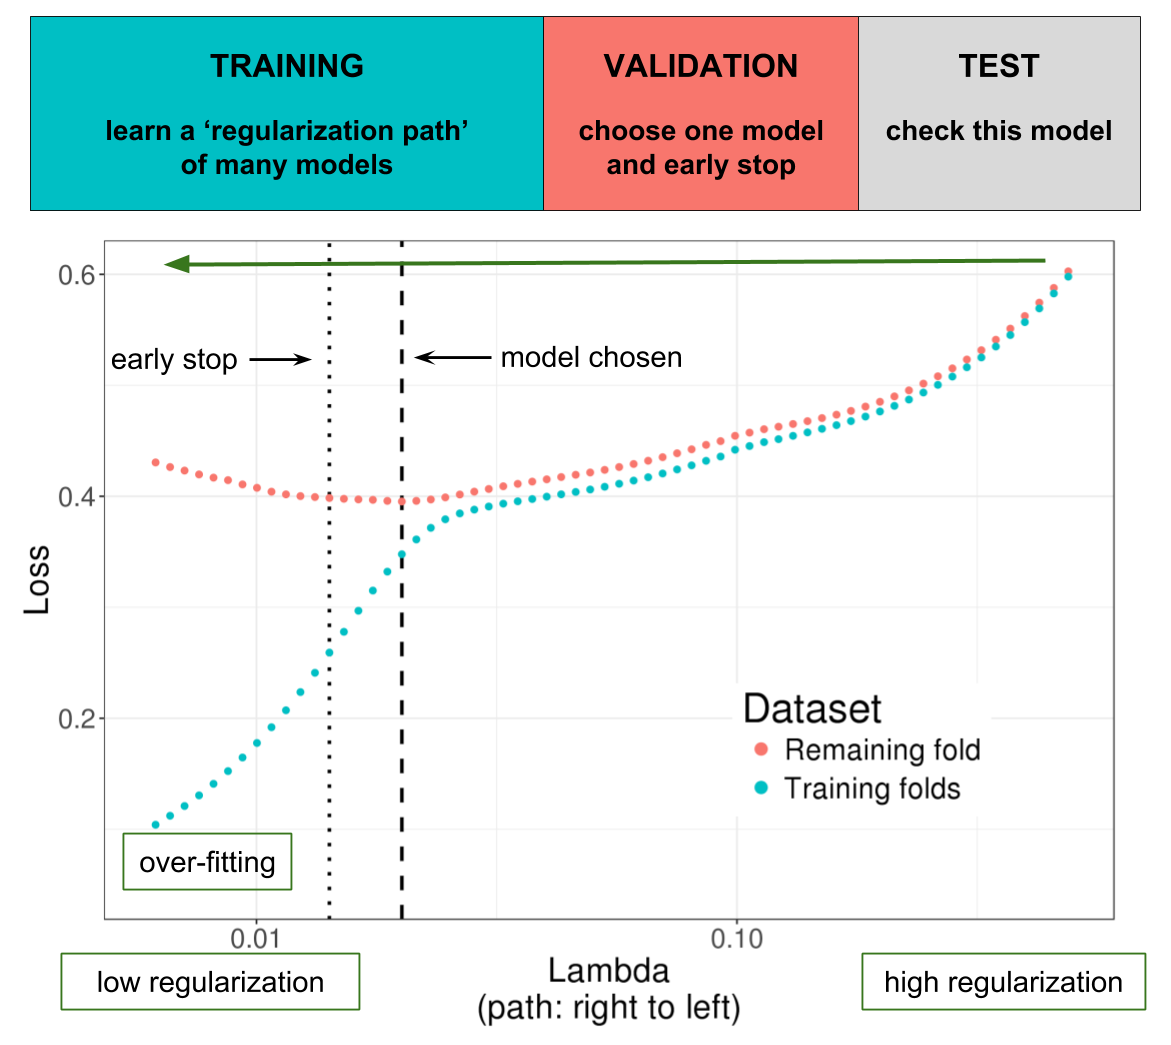
\includegraphics[width=0.85\textwidth]{simple-CMSA}}
	\caption{Illustration of one turn of the Cross-Model Selection and Averaging (CMSA) procedure (figure from \cite{prive2019efficient}). First, this procedure separates the training set in $K$ folds (e.g.\ 10 folds). 
		Secondly, in turn, each fold is considered as an inner validation set (red) and the other ($K - 1$) folds form an inner training set (blue). A ``regularization path'' of models is trained on the inner training set and the corresponding predictions (scores) for the inner validation set are computed. The model that minimizes the loss on the inner validation set is selected. Finally, the $K$ resulting models are averaged. 
		We also use this procedure to derive an early stopping criterion so that the algorithm does not need to evaluate the whole regularization paths, making this procedure much faster.}
	\label{fig:CMSA}
\end{figure}

Third, \cite{qian2020fast} recommend not to use scaled genotypes when applying lasso to genetic data. 
However, using scaled genotypes is common practice in genetics, and is the assumption behind models in popular software such as GCTA and LDSC \cite[]{yang2011gcta,bulik2015ld}.
Scaling genotypes assumes that all variants explain the same amount of variance and that low-frequency variants have larger effects on average.
\cite{speed2012improved} argued that this assumption might not be reasonable and proposed another model: $\mathbb{E}[h^2_j] \propto \left[p_j (1 - p_j)\right]^\nu$, where $h^2_j$ is the variance explained by variant $j$ and $p_j$ is its allele frequency. %Note that $\nu$ is usually termed $\alpha$ but we change the notation here to avoid confusion with the hyper-parameter $\alpha$ from elastic-net regularization.
In \cite{speed2017reevaluation}, they estimated $\nu$ to be between $-0.25$ and $-0.5$ for most traits.
Note that scaling genotypes by dividing them by their standard deviations as done by default in bigstatsr would correspond to using $\nu=-1$ while not doing any scaling as argued by \cite{qian2020fast} would correspond to using $\nu=0$.
Therefore, using a trade-off between these two approaches can provide higher predictive performance and is therefore recommended \cite[]{zhang2020improved}.
In the case of lasso regularization, using a different scaling can be obtained by using a different penalty for all variants, introducing a different penalty factor $\lambda_j$ for different variable $j$ in equation \eqref{eq:lasso}.
Using $\lambda_j=\left[p_j (1 - p_j)\right]^{-1}$ allows to effectively use unscaled genotypes; using different penalty factors is an option available in both bigstatsr and snpnet.
More recently, we have implemented a new parameter \texttt{power\_scale} to allow for different scalings when fitting the lasso in bigstatsr. Note that a vector of values to test can be provided, and the best-performing scaling is automatically chosen within the CMSA procedure.

%%%%%%%%%%%%%%%%%%%%%%%%%%%%%%%%%%%%%%%%%%%%%%%%%%%%%%%%%%%%%%%%%%%%%%%%%%%%%%%%

\section*{From theory to practice}

In previous sections, we discussed why we expect bigstatsr to be more efficient and to provide higher predictive performance than snpnet.
To practically support our claims, we now perform comparisons for the 4 real traits used in the UK Biobank analyses of \cite{qian2020fast}.

[TODO: REDO WITH THE SAME PHENO + SAME SPLIT AS IN THEIR PAPER]

For comparing similar models, we use a 10-fold CMSA procedure in bigstatsr, but also report the performance using only one training-validation split in bigstatsr (90\% training and 10\% validation). We use the same split to train snpnet.
Moreover, we use penalty factors to effectively use unscaled genotyped in bigstatsr, as performed by default in snpnet (see section Recommendations); note that this has become a direct option in recent versions.
We show that we get the same prediction when using unscaled genotypes and when using the same training-validation split for bigstatsr and snpnet (Figure \ref{fig:preds}).

[TODO: SHOWING PREDICTION FOR BOTH THE SAME FOLD AND CMSA + TIMING]

\begin{table}[h]
	\caption{[TODO: CAPTION]\label{tab:results}}
	\vspace*{0.5em}
	\centering
	\begin{tabular}{|l|c|c|c|c|c|}
		\multicolumn{1}{l|}{} & \multicolumn{2}{c|}{snpnet} & \multicolumn{3}{c|}{bigstatsr} \\
		\hline
		Trait & Perf. & Time & Perf. (1 fold) & Perf. (CMSA) & Time (CMSA) \\
		\hline
		Type 2 diabetes (T2D) & 62.27 & 78 min & 62.23 & 62.92 & 24 min \\
		\hline
	\end{tabular}
\end{table}

\begin{figure}[h]
	\centerline{\includegraphics[width=0.7\textwidth]{compare-preds}}
	\caption{Predictions from genetic data for T2D using either snpnet or bigstatsr (using one validation fold only).}
	\label{fig:preds}
\end{figure}

%%%%%%%%%%%%%%%%%%%%%%%%%%%%%%%%%%%%%%%%%%%%%%%%%%%%%%%%%%%%%%%%%%%%%%%%%%%%%%%%

\section*{Discussion}

We have shown both theoretically and empirically that bigstatsr provides faster and more accurate models than snpnet, and also made some recommendations on how to best use penalized regression for deriving polygenic scores based on very large individual-level genetic data.
Note that, in \cite{qian2020fast}, no comparison is made with bigstatsr in terms of predictive performance. The only comparison reported focuses on computation time and show that bigstatsr is slower than snpnet on a small synthetic dataset.
[TODO: WE DO IT AND DESCRIBE RESULTS]

\cite{qian2020fast} wrote that bigstatsr ``do not provide as much functionality as needed in [their] real-data application'', mainly because bigstatsr requires converting the input data and cannot handle missing values.
It is true that bigstatsr uses an intermediate format, which is a simple on-disk matrix format accessed via memory-mapping.
However, package bigsnpr provides fast parallel functions \texttt{snp\_readBed2} for converting from `.bed' files and \texttt{snp\_readBGEN} for converting from imputed `.bgen' files, the two formats used by the UK Biobank.
For example, it took 6 minutes only to read from the UK biobank `.bed' file used in this paper. We then used function \texttt{snp\_fastImputeSimple} to impute by the mean in 5 minutes only, which is also the imputation strategy used in snpnet.
When reading imputed dosages instead, it takes less than one hour to access and convert 400K individuals over 1M variants using function \texttt{snp\_readBGEN} with 15 cores, and less than three hours for 5M variants.
When available, we recommend to directly read from `.bgen' files to get dosages from external reference imputation.
As for package snpnet, it uses the PLINK 2.0 `.pgen` format, which is still under active development (in alpha testing, see \url{https://www.cog-genomics.org/plink/2.0/formats#pgen}).
This format is not currently provided by the UK Biobank, and can therefore be considered as an intermediate format as well.

\cite{qian2020fast} also points out the lack of flexibility of bigstatsr because it handles linear and logistic regression but not Cox regression, and can only use standardized variables.
While it is true that Cox regression is not yet implemented in bigstatsr, it is one of the regression for which it is easy to derive strong rules \cite[]{tibshirani2012strong} so it would be relatively easy to implement it in bigstatsr. Anyway, in some upcoming work, we will show that there may be a better alternative to Cox regression for genetic prediction and association.
As for scaling, we have seen how to effectively get unstandardized genotypes using penalty factors in section Recommendations, and we actually recommend to use an in-between scaling, or to test different scaling values using the new parameter \texttt{power\_scale} in bigstatsr.
Finally, when we developed R packages bigstatsr and bigsnpr for analyzing large scale genetic data, we separated functions in two packages because some functions are not specific to genetic data (the ones in bigstatsr).
Therefore, when using our on-disk matrix format, one can store e.g.\ other omics data and also have access to a broad range of analysis tools provided by bigstatsr, e.g.\ ultra-fast penalized regressions, association studies and principal component analysis without any extra coding \cite[]{prive2018efficient}.

To sum up, we have found the BASIL approach derived in \cite{qian2020fast} to be a clever approach to try to alleviate the I/O problem of other penalized regression implementations for very large datasets.
Yet, we use a simpler and more pragmatic alternative in bigstatsr and show that this leads to faster fitting of penalized regression in bigstatsr.
Moreover, because we make use of the full training set, we also achieve higher predictive performance with bigstatsr compared to snpnet.


%%%%%%%%%%%%%%%%%%%%%%%%%%%%%%%%%%%%%%%%%%%%%%%%%%%%%%%%%%%%%%%%%%%%%%%%%%%%%%%%

\clearpage
%\vspace*{5em}

\section*{Software and code availability}

[TODO: EXPORT CODE FROM CLUSTER] 

%All code used for this paper is available at \url{https://github.com/privefl/paper-ldpred2/tree/master/code}.
%The newest version of R package bigsnpr can be installed from GitHub (see \url{https://github.com/privefl/bigsnpr}).
A tutorial on fitting penalized regressions with R package bigstatsr is available at \url{https://privefl.github.io/bigstatsr/articles/penalized-regressions.html}. 

\section*{Acknowledgements}

This research has been conducted using the UK Biobank Resource under Application Number 41181.
Authors would also like to thank GenomeDK and Aarhus University for providing computational resources and support that contributed to these research results.

\section*{Funding}

F.P. and B.V.\ are supported by the Danish National Research Foundation (Niels Bohr Professorship to Prof. John McGrath), and also acknowledge the Lundbeck Foundation Initiative for Integrative Psychiatric Research, iPSYCH (R248-2017-2003).

\section*{Declaration of Interests}

The authors declare no competing interests.

%%%%%%%%%%%%%%%%%%%%%%%%%%%%%%%%%%%%%%%%%%%%%%%%%%%%%%%%%%%%%%%%%%%%%%%%%%%%%%%%

\clearpage

\bibliographystyle{natbib}
\bibliography{refs}

%%%%%%%%%%%%%%%%%%%%%%%%%%%%%%%%%%%%%%%%%%%%%%%%%%%%%%%%%%%%%%%%%%%%%%%%%%%%%%%%


\end{document}
